\chapter{AI Component Design}
\label{chap:ai-component-design}

% \section{Software Development Methodology}
% \label{section:software-development-methodology}
% <TIP: Describe your software development methodology in this section. />

% \section{Technology Stack}
% \label{section:technology-stack}
% <TIP: Describe your technology stack here. See the following example from ThaiProgrammer.org />
% \begin{figure}[h]
%     \centering
%     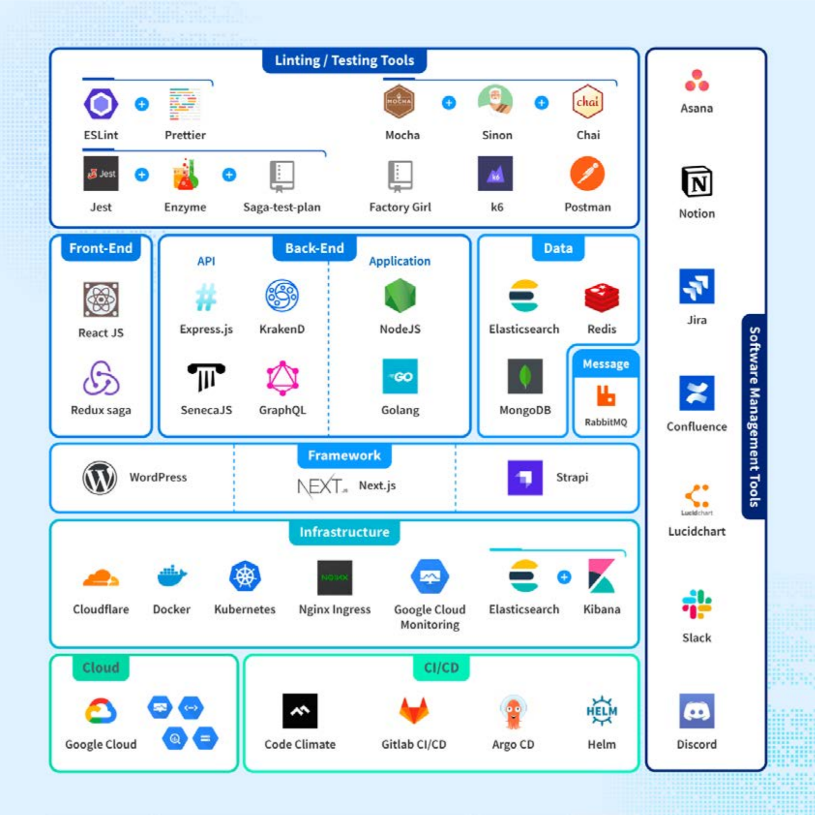
\includegraphics[width=0.5\textwidth]{examples/tech-stack.png}
%     \caption{Example technology stack}
% \end{figure}

% \section{Coding Standards}
% \label{section:coding-standards}
% <TIP: Describe your coding standard for this project here. />

% \section{Progress Tracking Report}
% \label{section:progress-tracking-report}
% <TIP: Show that you have been working on this project overtime.
% It can be in the form of a burndown chart or a contribution graph from GitHub./>

\section{Business Context \& AI Integration}

\label{section:business-context-ai-integration}
\begin{figure}[H]
    \centering
    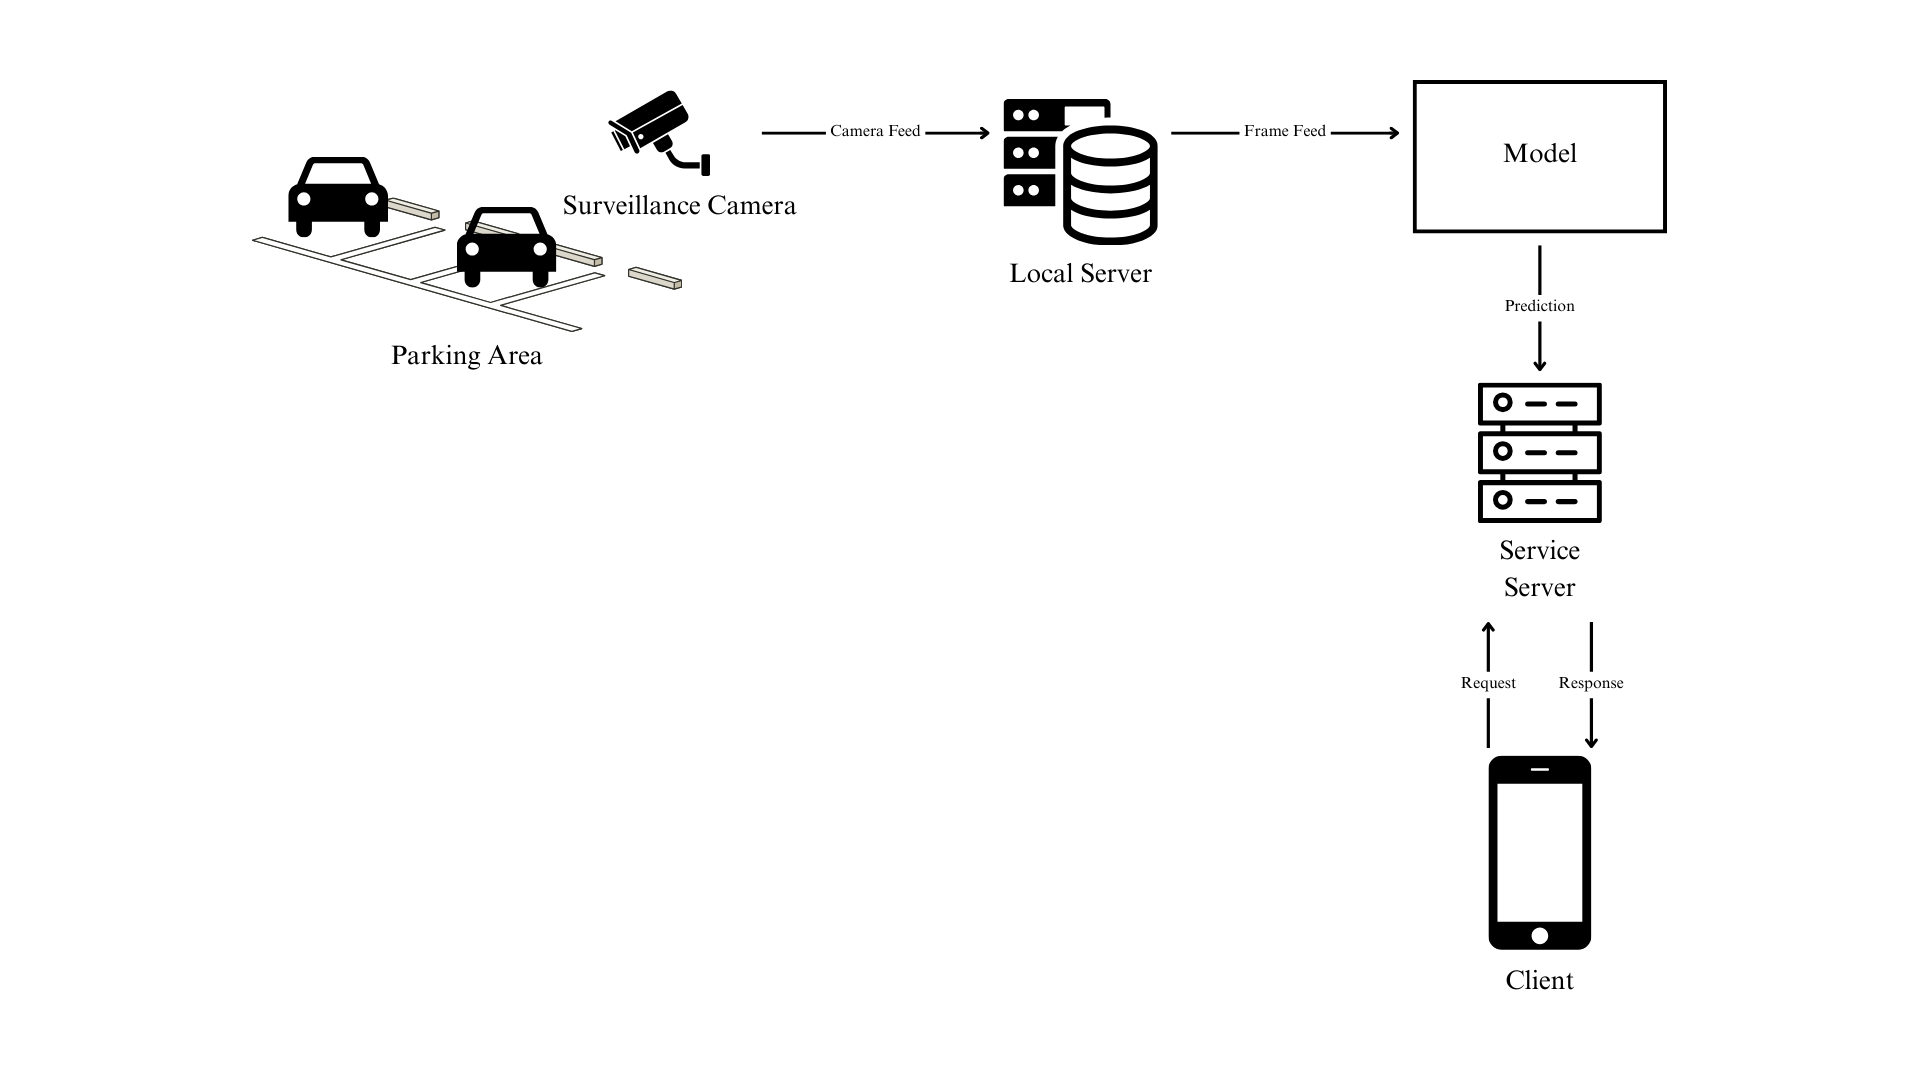
\includegraphics[width=\textwidth,keepaspectratio]{diagrams/system-flow/overview-system-flow.png}
    \caption{Overview System Flow}
    \label{fig:overview-system-flow}
\end{figure}

\begin{figure}[H]
    \centering
    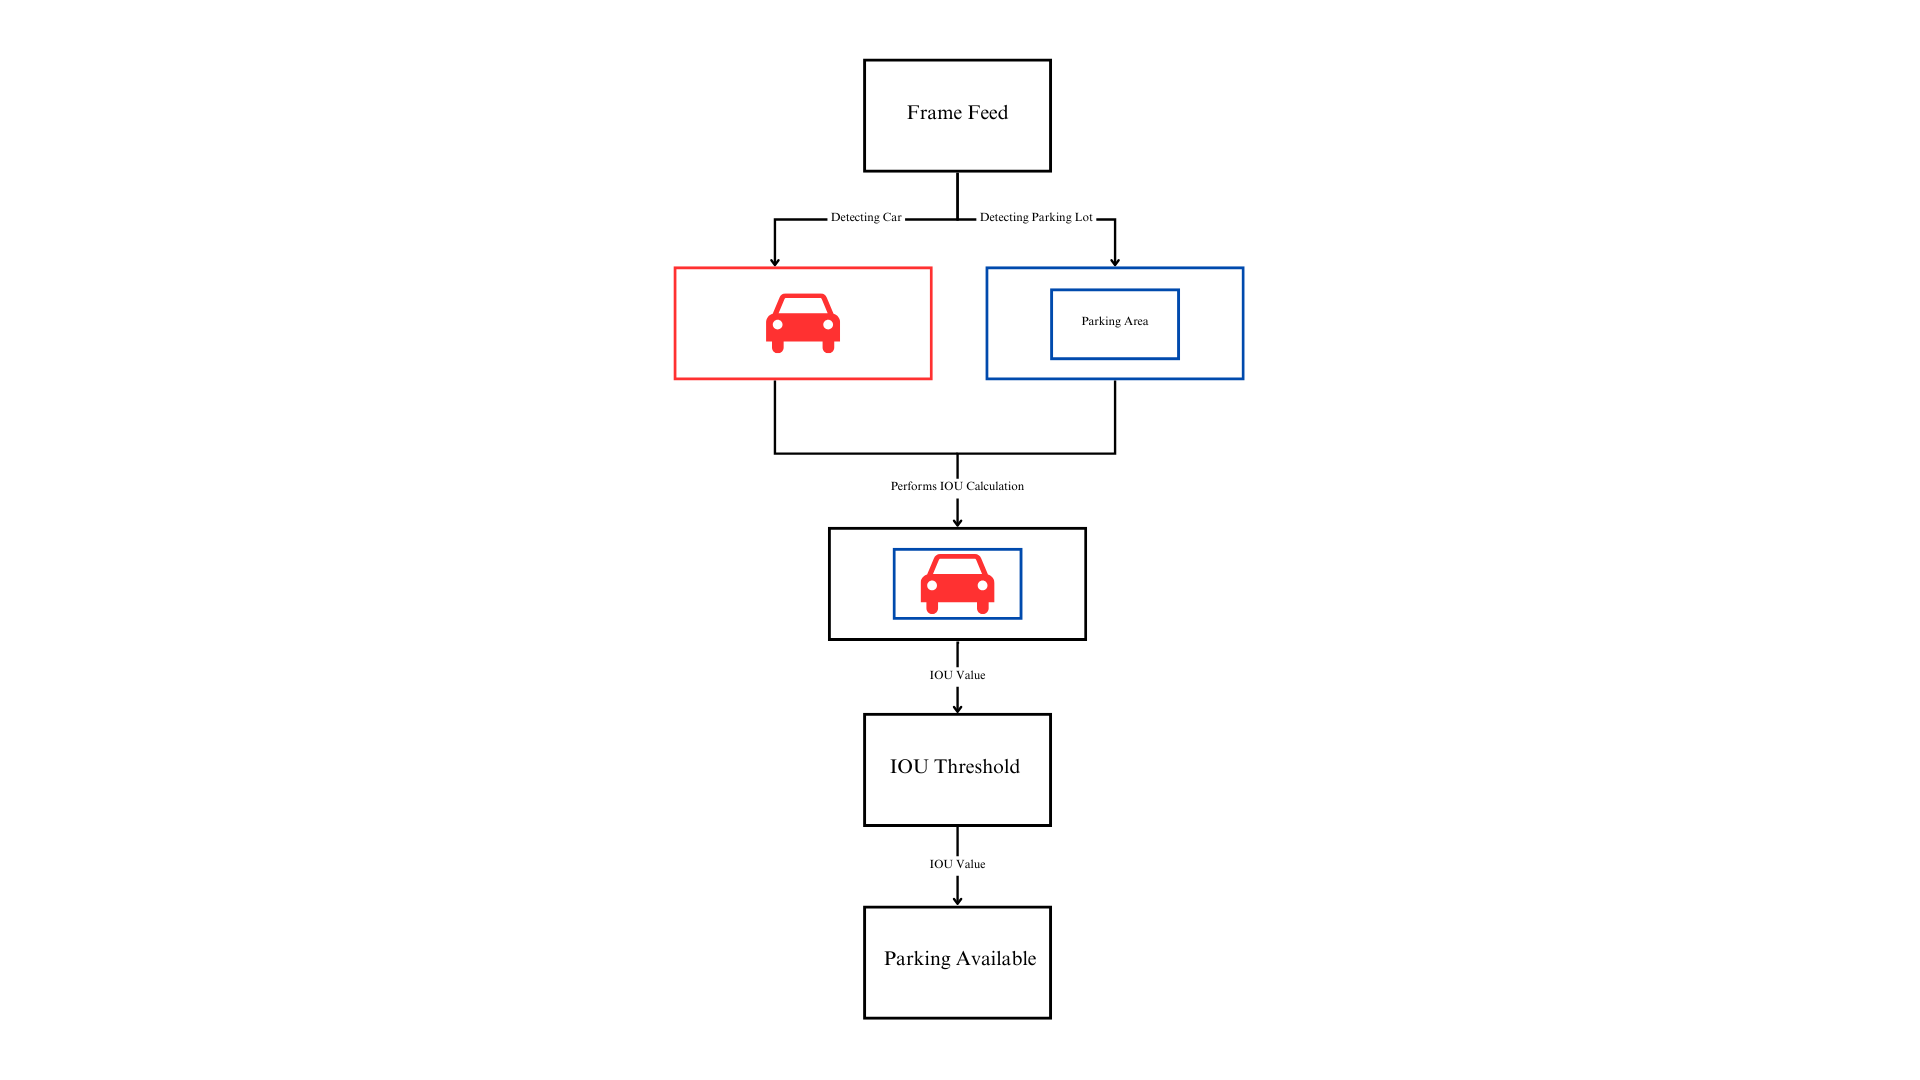
\includegraphics[width=\textwidth,keepaspectratio]{diagrams/system-flow/model-flow.png}
    \caption{Detection Model Flow}
    \label{fig:model-flow}
\end{figure}


KU Parking has integrated AI for the detection of available parking spots. Figure \ref{fig:overview-system-flow} provides a system overview: surveillance cameras monitor the parking area, feeding video to a local surveillance footage server. Periodically, individual frames from the video stream are extracted and processed by the model (as outlined in Figure \ref{fig:model-flow}). The model performs object detection to locate both cars and parking spaces within the image. Subsequently, it calculates the Intersection over Union (IoU), a metric quantifying the overlap between each detected vehicle's bounding box and the defined area of a parking spot. By comparing the IoU against a set threshold, the system determines if a vehicle significantly occupies a parking space, thus indicating its availability. This output is served to the client by the service server.

By integrating a detection model, KU Parking can reduce the cost of installing a parking indication system by leveraging existing infrastructure. To inform users, parking availability requires continuous monitoring, as the availability and usage of parking spots can change throughout the day. The model helps automate this continuous monitoring process by analyzing feeds, providing up-to-date information on parking spot occupancy. The incorrect detections typically result in minor user frustration rather than significant damage.

\section{Goal Hierarchy}
\label{section:goal-hierarchy}
<TIP: Describe your coding standard for this project here. />

\section{Task Requirements Analysis Using AI Canvas}
\label{section:task-requirement-analysis-using-ai-canvas}
<TIP: Describe your coding standard for this project here. />


\section{User Experience Design with AI}
\label{section:user-experience-with-ai}
<TIP: Describe your coding standard for this project here. />
